%% LyX 2.0.6 created this file.  For more info, see http://www.lyx.org/.
%% Do not edit unless you really know what you are doing.
\documentclass[oneside,english]{amsart}
\usepackage[T1]{fontenc}
\usepackage[latin9]{inputenc}
\usepackage{amsthm}
\usepackage{fullpage}
\usepackage{graphicx}
%\usepackage{enumerate}
\usepackage{float}
\usepackage{amsmath}
\usepackage{url} % click on urls 

\usepackage[parfill]{parskip}
\usepackage{hyperref}
\usepackage{xcolor}

\usepackage{enumitem}

\makeatletter
%%%%%%%%%%%%%%%%%%%%%%%%%%%%%% Textclass specific LaTeX commands.
\numberwithin{equation}{section}
\numberwithin{figure}{section}


\makeatother

\usepackage{babel}
\begin{document}
\pagenumbering{gobble}


\hspace{1cm} \\
\vspace{-3.5cm} 

\centerline{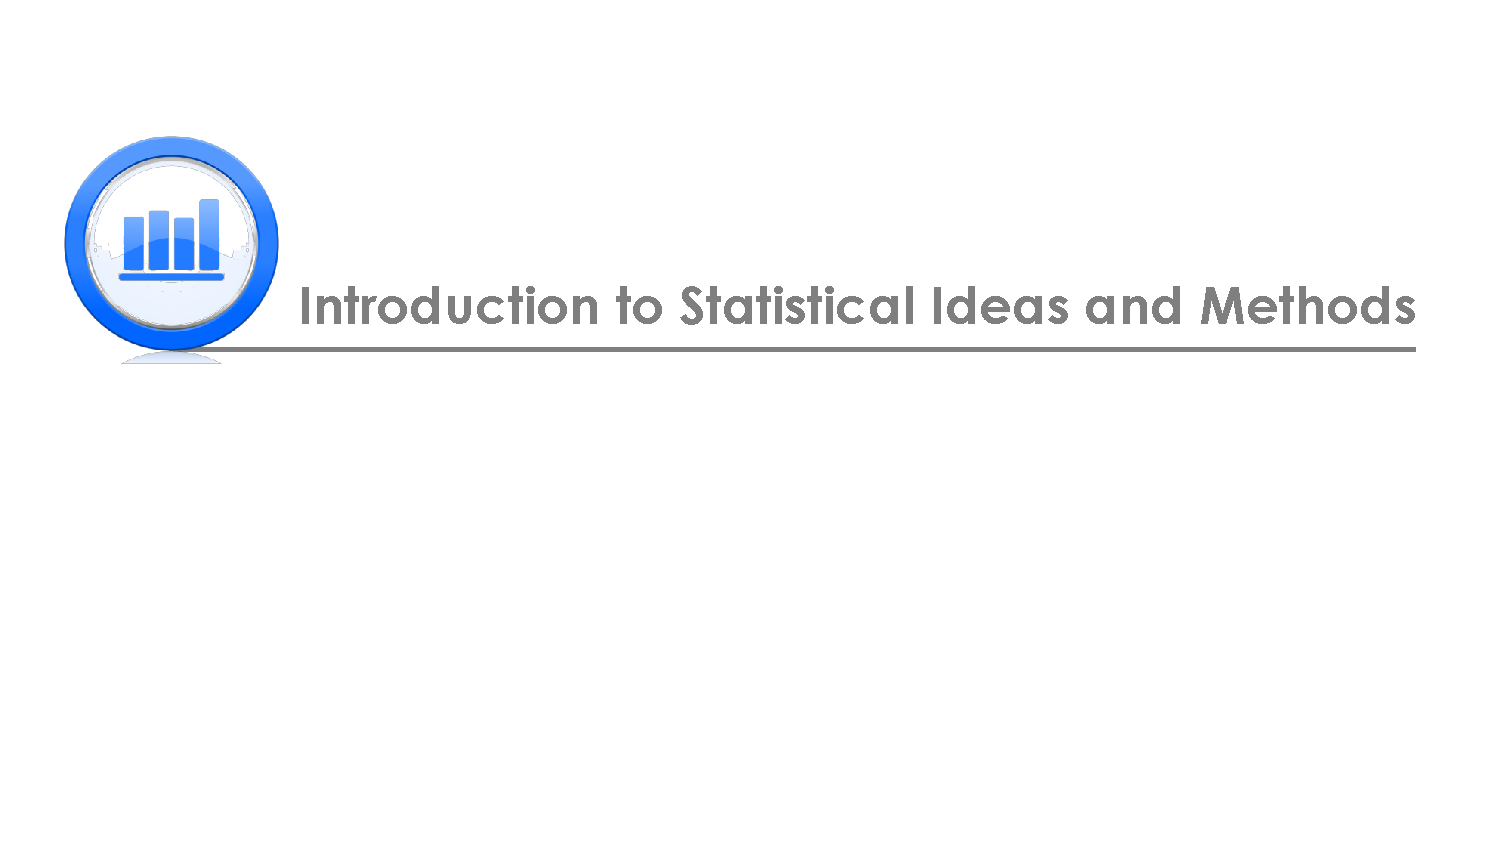
\includegraphics[width=1.1\textwidth]{../../figures/headerfinal.pdf}}

\vspace{.5cm}


%\centerline{{\large{Statistical Tests II: Power App}}} \normalsize  \vspace{.2cm} % Video title
\title{Visualizing the Skeleton Data}

\maketitle
Recall that the skeleton data were collected in order to assess the
accuracy of methods used by anthropologists to estimate age at death.
The Visualizing Skeleton Data RShiny app lets us quickly inspect the
data by producing a number of helpful visualizations. In this exercise
we will do the first stages of an exploratory analysis of these data.
\begin{enumerate}
\item As a warm-up, make a histogram of the age variable by selecting ``histogram''
under plot type and ``Age'' under variable of interest. What does
selecting a subgroup option do?
\vspace{3cm}
\item Change the plot type to ``pie chart''. What are the possible variables
of interest that can be plotted? Are they same as the for the ``box
plot'' plot type? Why?
\vspace{3cm}
\item  Real world data often come with mistakes or mislabellings. The skeleton
data includes BMI as both a quantitative variable and as a categorical
variable. Try several different ways of plotting the quantitative
BMIquant separated by subgroup BMIcat. Do you notice anything unusual?
\vspace{3cm}
\item  If our data were overwhelmingly from males or overwhelmingly from
obese people we might miss seeing effects due to these factors. This
is because if one group is strongly overrepresented then there is
limited data that can be used to differentiate an effect specific
to that group. Try producing a pie chart and a bar chart for the categorical variables. Does it seem like any group is strongly overrepresented or underrepresented? 
\vspace{3cm}
\item  Pie charts are popular in some groups but not amongst statisticians.
Try producing pie charts of Sex and BMIcat and use the pie charts
to estimate the relative frequencies of each category visually. The
true relative frequencies are shown in the Data Summary under the
chart. Were your estimates accurate?
\vspace{3cm}
\item  Observational data with many potential contributing factors can sometimes
lead us to confuse the source of observed effects. For example, if
almost all of the obese people in the dataset were very old then we
might confound inaccurate predictions due to age and obesity (ie.
we might attribute age affects to obesity and vice versa). Use the
plots to explore whether this phenomena is present in our data set.
Are there comparisons you would like to make that are not possible
with the plotting available in the app?
\vspace{3cm}
\item  What is the average BMI for females in this data set? What is the
average BMI for males?
\vspace{3cm}
\item  The dataset includes estimates from two different strategies: Di Gangi
et al. (DGestimate) and Suchey-Brooks (SBestimate). For each of the
estimation strategies decide whether the method tends to overestimate
or underestimate age of death. The errors in estimation ($|\mbox{True Age}-\mbox{Estimated Age}|$) are given
as DGerror and SBerror respectively. What plots are most useful for
assessing this? If you were an anthropologist how might you make use
of this information?
\vspace{3cm}
\item  For each of the estimation strategies, does it seem that body mass
or sex substantially impacts the size of the error? How about the
variability of the estimate? What kind of plots are useful for assessing
this?
\vspace{3cm}
\item  In practical terms an anthropologist would just like to know which
of these age estimation methods they should use. Thinking ahead, what
further exploratory analysis might be useful before making a preliminary
recommendation? Are there any additional visualizations or plots that
you think should be produced?\end{enumerate}

\end{document}
